\documentclass[12pt,a4paper,german]{report}
\usepackage{geometry}
\geometry{a4paper, top=25mm, left=25mm, right=25mm, bottom=25mm, headsep=10mm, footskip=12mm}
\usepackage[utf8]{inputenc}
\usepackage{titlesec}
\usepackage{blindtext}
\usepackage{hyperref}
\usepackage{babel}
\usepackage{titlepic}
\usepackage{graphicx}
\usepackage{algorithm}
\usepackage{amsmath}
\usepackage{amsfonts}
\usepackage{mathptmx}
\usepackage{wrapfig}
\usepackage[onehalfspacing]{setspace}
\usepackage[noend]{algpseudocode}
\graphicspath{ {./images/} }

\titleformat{\chapter}{\normalfont\huge\bfseries}{\thechapter.}{20pt}{\huge\bfseries}

\newcommand{\floor}[1]{\left\lfloor #1 \right\rfloor}
\newcommand{\ceil}[1]{\left\lceil #1 \right\rceil}

%%%%%%%%%%%%%%%%%%%%%%%%%%%%%%%%%%%%%%%%%%%%%%%%%%%%%%%%%%%%%%%%%%%%%%%%%%%%%%%%

\begin{document}

\begin{titlepage}
  \centering
  
\includegraphics[width=0.05\textwidth]{ktzh}\par
  {\scshape\LARGE Berufsmaturitätsschule Zürich \par}
  \vspace{0.25cm}
  {\scshape\Large Berufsmaturitätsarbeit \par}
  {\scshape Technik,  Architektur,  Life  Sciences \par}
  \vspace{0.50cm}
  {\huge\bfseries Pathfinding-Algorithmen: Einführung und Vergleich mittels einer Webapplikation \par}
  \vspace{0.5cm}
  Oberthema: \textsc{Mobilität} \\
  \vspace{0.5cm}
  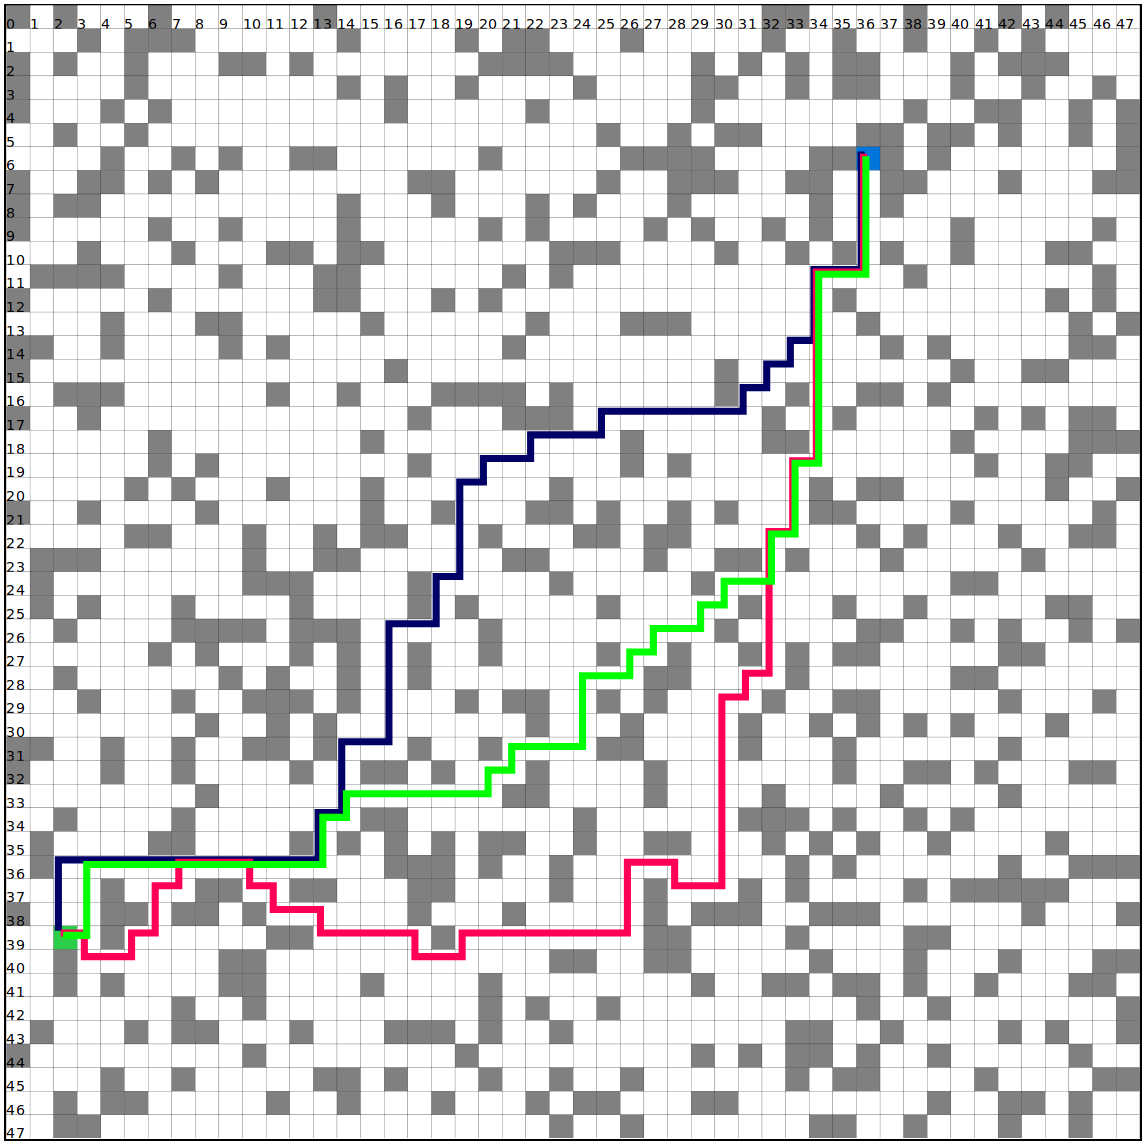
\includegraphics[width=0.65\textwidth]{cover2}\par
  \vspace{0.5cm}
  \begin{tabular}[t]{c@{\extracolsep{4em}}c} 
  \large\textsc{Adrian Stoop} & \large\textsc{Severin Fürbringer} \\ 
  adrian-stoop@gmx.ch & severin@fsfe.org\\
  EVT18a & EVT18a
  \end{tabular}
  \vfill
  \vspace{0.25cm}
  \large\textsc{Dr. Jürg Pöttinger}\\
  \normalsize{Begleitperson}
  \vspace{0.25cm}
  \vfill
  {1. Februar, 2019 \par}
\end{titlepage}


\renewcommand{\abstractname}{Abstract}
\begin{abstract}
Pathfinding-Algorithmen sind Programmabläufe, welche in der Wirtschaft in vielen Anwendungen vorkommen, wie zum Beispiel in Video Spielen, Simulationen oder der Automobilindustrie. 
Im Rahmen dieser Berufsmaturitätsarbeit wird eine Webapplikation entwickelt, die den Benutzer in das Thema der Pathfinder-Algorithmen einführt und einen interaktiven Vergleich von drei ausgewählten Pathfindern ermöglicht und dazu Messungen mit drei Merkmalen macht. Im Rahmen der Arbeit wählen wir den A*, BestFirst, und BreadthFirstFinder.
Die Webapplikation generiert für den Vergleich ein Zufallslabyrinth, markiert Start- und Endpünkte und lässt mehrere Vergleiche in Serie geschaltet zu.
Mithilfe des Pathfinder-Vergleichers werden im Rahmen der Arbeit auch Statistiken erstellt und ausgewertet und im schriftlichen Teil die Funktionsweisen der Pathfinder erläutert.
\\
  Die Webapplikation ist unter \url{https://bma.fuerbringer.info} zugänglich. Der dazugehörige Quellcode ist frei unter \url{https://github.com/fuerbringer/bma} erhältlich.
\end{abstract}


\tableofcontents{}

% START THESIS CONTENT
%%%%%%%%%%%%%%%%%%%%%%%%%%%%%%%%%%%%%%%%%%%%%%%%%%%%%%%%%%%%%%%%%%%%%%%%%%%%%%%%

\chapter{Einleitung}

%%%%%%%%%%%%%%%%%%%%%%%%%%%%%%%%%%%%%%%%%%%%%%%%%%%%%%%%%%%%%%%%%%%%%%%%%%%%%%%%
\chapter{Realisierung}
Dieser Abschnitt soll dazu verhelfen, die technischen Entscheidungen und Schritte zu erläutern und es möglich zu machen, die Kernfunktionen des Projekts zu reproduzieren. Leser, die diese Applikation, oder Teile davon, anderweitig einsetzen möchten, beziehen sich zusätzlich auf den frei verfügbaren Quellcode\cite{bma} des gesamten Projekts.
\section{Konzept}
Die Konzipierung dieser Webapplikation verlangte einige technische und gestalterische Entscheidungen. 
Einerseits musste die Programmiersprache und Struktur der Applikation geplant werden und andererseits auch das eigentliche Aussehen der Benutzeroberfläche der Webapplikation. 
Auf diese zwei wesentlichen Aspekte wird in diesem Abschnitt eingegangen.
\subsection{Pathfinding.js}
Eine korrekte Implementation der ausgewählten Pathfinder sind Voraussetzung für das Projekt. 
Daher wurde, um diese Voraussetzung zu erfüllen, die frei verfügbare Implementation PathFinding.js \cite{pfjs} verschiedener Pathfinder ausgewählt.
\subsection{Programmierwerkzeuge}
Die vorhandenen Fachkenntnisse und Erfahrungen schlugen für die Implementierung entweder PHP oder JavaScript als mögliche Programmiersprachen vor. 
Zum Entscheid massgebend war, dass die Programmbibliothek PathFinding.js \cite{pfjs}, welche in unserer Arbeit eine wichtige Rolle spielt, in JavaScript implementiert wurde. 
Durch den Einsatz von JavaScript im Front-End und im Back-End, wäre es möglich die Pathfinder Berechnungen beliebig auf dem Rechner des Nutzers und auch auf dem Rechner des Servers auszuführen. Aus diesen Gründen wurde für das Front- und Back-End JavaScript ausgewählt.
Folgend werden die wichtigsten Technologien unserer Webapplikation aufgelistet\footnote{Eine komplette Auflistung inklusive der abhängenden Programmbibliotheken macht wenig Sinn, vor allem da unser Quellcode frei ersichtlich ist.}.

\begin{description}
  \item [Programmiersprache] JavaScript mit Einbindung von PathFinding.js \cite{pfjs}
  \item [Webserver-Software] Express\footnote{Express Webserver für Node Webapplikationen, \url{https://expressjs.com/}, Stand: \today} übernimmt die Ausführung von JavaScript im Back-End.
  \item [Quellcode-Hosting] GitHub\footnote{GitHub, \url{https://github.com/}, Stand: \today}. Der Quellcode unser Webapplikation ist frei unter\\ \url{https://github.com/fuerbringer/bma} zugänglich.
  \item [Webhosting] Die Vultr\footnote{Vultr - The Infrastructure Cloud™, \url{https://vultr.com/}, Stand: \today}-Cloud dient als Hosting-Provider. Prinzipiell kann die Webapplikation jedoch auf beliebigen Unix und GNU/Linux Servern gehostet werden.
\end{description}

\subsection{Konzipierung der Benutzeroberfläche}
Als Webapplikation muss unsere Arbeit deren Nutzen dem Benutzer ausreichend klar machen. 
Umsomehr ist dies von Bedeutung, da die Webapplikation frei zugänglich ist und daher auch Besucher die Idee der Webapplikation verstehen sollten. 
Aus diesem Grund wurde unsere Webapplikation für den Nutzer einführend gestaltet. 
Das heisst, dass der Benutzer beim Aufruf der Webapplikation zunächst auf einer Willkommensseite landet, die ihn wiederum zu einer Einführung in das Thema und Ziel der Arbeit führt. 
Nach der Einführung kann der Benutzer in der Visualisierung mit einzelnen Pathfindern erste Erfahrungen machen. 
Im Abschluss kommt der Benutzer zum Hauptteil der Arbeit, dem Pathfinding-Vergleicher. 
Ziel dieser Struktur ist, dass jede Person wenigstens einen Einblick in die Welt der Pathfinding-Algorithmen erhält und über das nötige Wissen verfügt, das Ziel des Pathfinding-Vergleichers zu verstehen.
\begin{figure}[H]
  \centering
  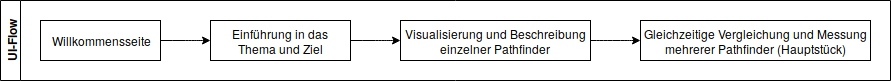
\includegraphics[width=16cm]{uiflow}
  \caption[Struktur der Webapplikation.]{Webapplikationsstruktur. Quelle: Eigenleistung}
  \label{fig:uiflow}
\end{figure}

\clearpage

\subsubsection{Einführungs- und Willkommensseite}
Die Einführungsseite erklärt dem Benutzer was Algorithmen sind und führt ihn anschliessend mit einfachen Beispielen in das Thema der Pathfinder ein. Zuletzt werden die Ziele der Arbeit aufgelistet.
\begin{figure}[H]
  \centering
  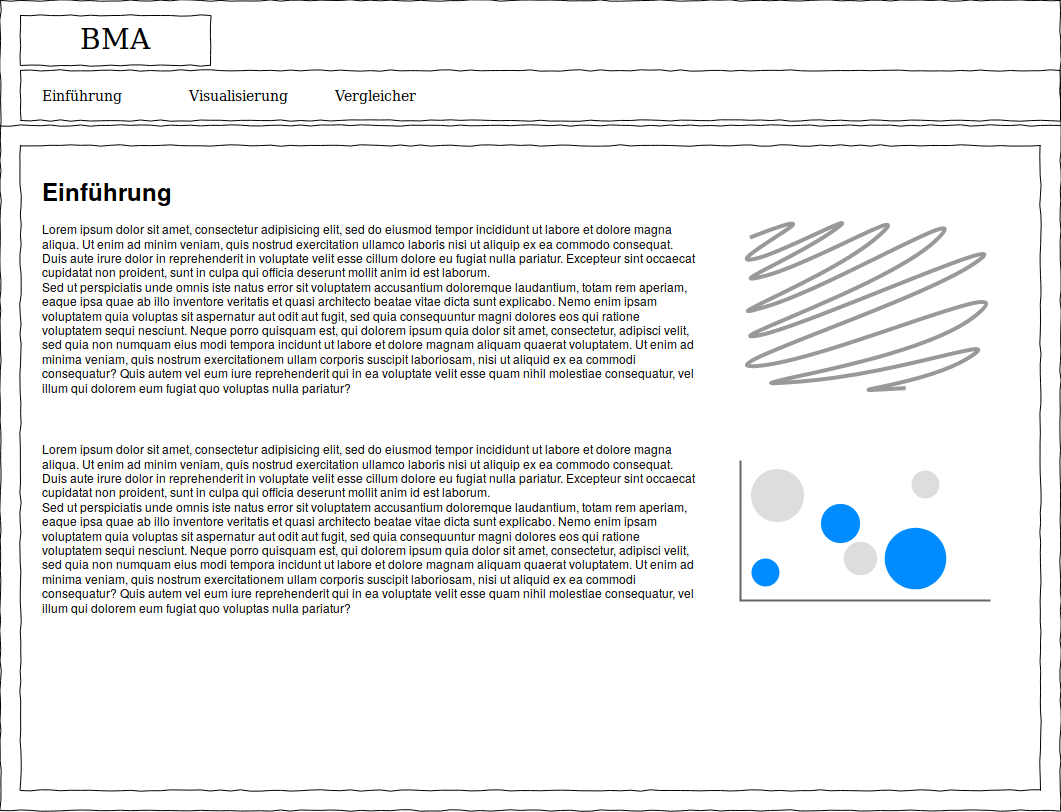
\includegraphics[width=16cm]{einfuehrung1}
  \caption[Konzept der Einführungsseite.]{Einführungsseite. Quelle: Eigenleistung}
  \label{fig:einfuehrung1}
\end{figure}

\clearpage

\subsubsection{Visualisierung der Pathfinder}
Nach der Einführung erhält der Benutzer die Möglichkeit mit einzelnen Pathfindern zu experimentieren. Dazu kann er auch verschiedene Parameter anpassen. Dies ist die Vorstufe zum Pathfinder-Vergleicher, da hier nochmals die einzelnen Pathfinder auf ihre Eigenschaften beschrieben werden.
\begin{figure}[H]
  \centering
  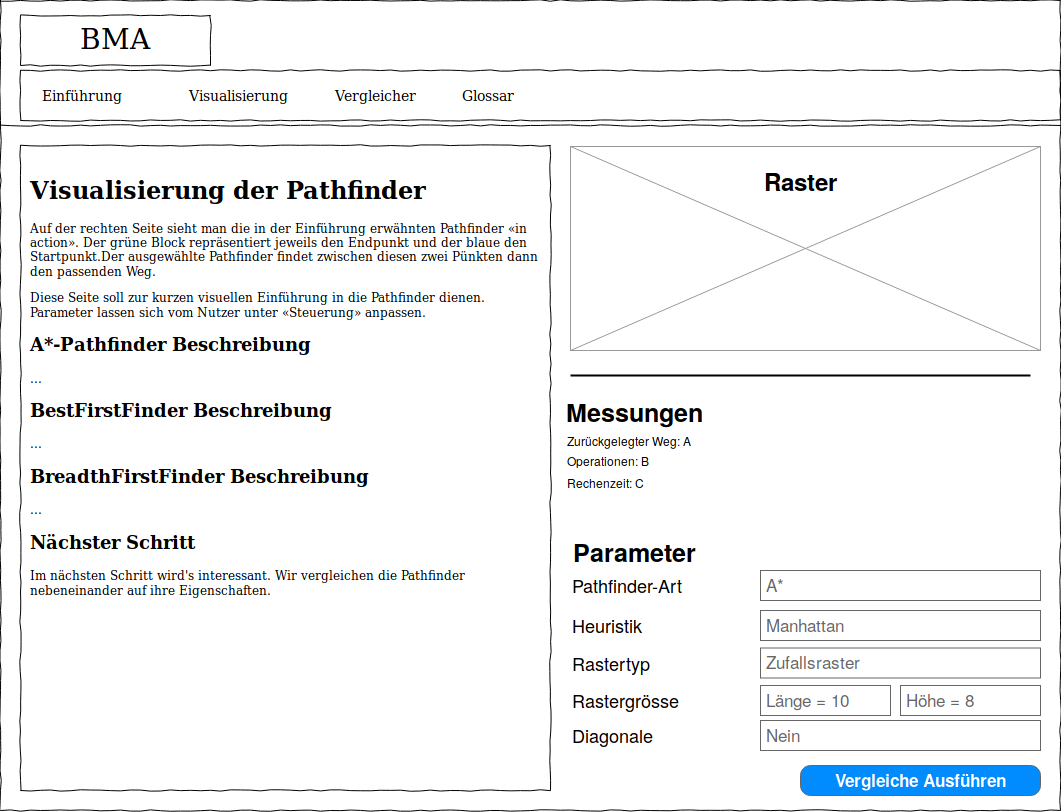
\includegraphics[width=16cm]{visualisierung1}
  \caption[Benutzeroberflächenkonzept des Pathfinding-Visualisierers.]{Benutzeroberflächenkonzept Visualisierer. Quelle: Eigenleistung}
  \label{fig:gui_konzept_visualizer}
\end{figure}

\clearpage

\subsubsection{Vergleich der Pathfinder}
Als Herzstück der Arbeit ermöglicht der Pathfinder-Vergleicher dem Nutzer die in unserer Arbeit ausgewählten Pathfinder zu vergleichen. Hier werden, gleich wie beim Visualisierer, zuerst vom Benutzer die Parameter gewählt. Die parallel ausgeführten Resultate mit Informationen über die Rechenzeit, zurückgelegten Weg und Operationen, sind dann interaktiv anwählbar. Gleichzeitig wird auch unter ``Resultate'' unten links das Total aller Vergleiche akkumuliert, damit ein Gesamteindruck verschaffen werden kann. Die Resultate dieser Seite dienen im Statistikteil als Datenquelle.

\begin{figure}[H]
  \centering
  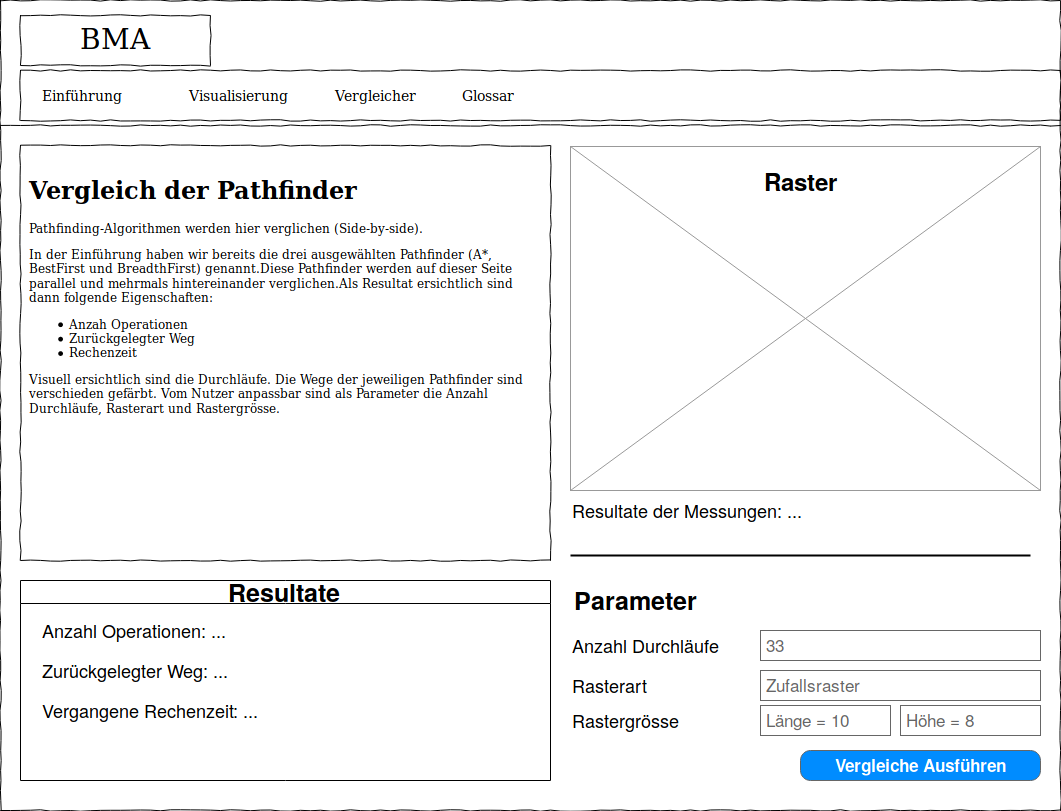
\includegraphics[width=16cm]{konzept1}
  \caption[Benutzeroberflächenkonzept des Pathfinder-Vergleichers.]{Benutzeroberflächenkonzept Vergleicher. Quelle: Eigenleistung}
  \label{fig:gui_konzept_comparator}
\end{figure}

\section{Implementierung des Vergleichers}
Vor allem für die statistischen Auswertungen ist es von Bedeutung zu wissen, wie der Vergleicher zu den Resultaten kommt und die Berechnungen durchführt. Um an die statistischen Merkmale zu gelangen, musste je nach Merkmal die Webapplikation oder PathFinding.js erweitert werden.

\subsection{Raster}
Pathfinder benötigen einen Raum, um ihre Arbeit zu verrichten. Folglich wird erläutert, wie diese Räume im Quellcode der Arbeit implementiert wurden.
Die Implementation der Pathfinding-Algorithmen von PathFinding.js erwartet als Raum eine Liste mit beispielsweise $8\times8$ Zellen: \\
\begin{center}
$[(0,0),(1,0),(2,0),(3,0),(4,0),(5,0),(6,0),(7,0)]$\\
$[(0,1),(1,1),(2,1),(3,1),(4,1),(5,1),(6,1),(7,1)]$\\
$[(0,2),(1,2),(2,2),(3,2),(4,2),(5,2),(6,2),(7,2)]$\\
$[(0,3),(1,3),(2,3),(3,3),(4,3),(5,3),(6,3),(7,3)]$\\
$[(0,4),(1,4),(2,4),(3,4),(4,4),(5,4),(6,4),(7,4)]$\\
$[(0,5),(1,5),(2,5),(3,5),(4,5),(5,5),(6,5),(7,5)]$\\
$[(0,6),(1,6),(2,6),(3,6),(4,6),(5,6),(6,6),(7,6)]$\\
$[(0,7),(1,7),(2,7),(3,7),(4,7),(5,7),(6,7),(7,7)]$
\end{center}
Zu beachten ist, dass die obige Liste pro Element (Zelle) lediglich die Koordinate $(x,y)$ als Eigenschaft aufweist. Weitere Eigenschaften pro Zelle, wie die Wandeigenschaft, werden in späteren Abschnitten erwähnt.
Diese Art von Raster ist bei der Darstellung von Pixelmatrizen und sonstigen computergrafikorientierten Anwendungen üblich. 
Man kann sich diese Anordnung auch als den vierten Quadranten eines kartesischen Koordinatensystems vorstellen, dessen $y$-Koordinate ihren Absolutwert annimmt. 
Des Weiteren gilt $x \in \mathbb{N}$ und $y \in \mathbb{N}$. 
Daraus folgt, dass Zwischenschritte nicht möglich sind, beispielsweise das Ziel nicht die Koordinate $(\frac{1}{2},\frac{42}{11})$ annehmen kann. Ein weiteres Beispiel dafür wären die Pixel eines gewöhnlichen Monitors, denn einen Bruchteil eines Pixels anzusteuern ist ebenfalls nicht möglich.
Benötigt man eine derartige Präzision, erhöht man dazu am besten die Auflösung des Raums. Es folgt eine Abbildung eines zweidimensionalen leeren Raumes der oben gegebenen Liste.
\begin{figure}[H]
  \centering
  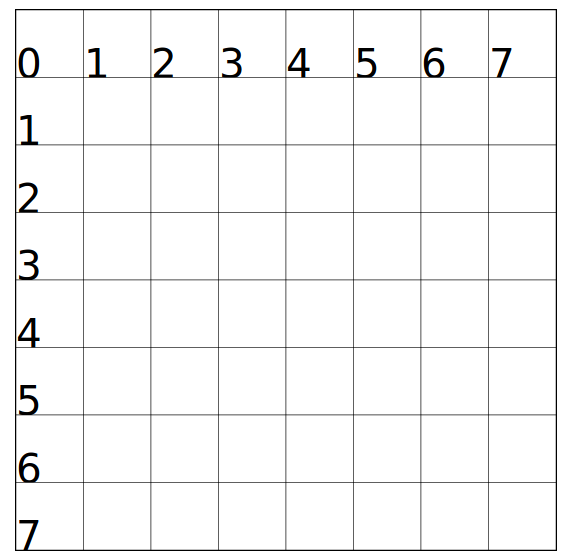
\includegraphics[width=8cm]{grid1}
  \caption[Ein von unserer Webapplikation generiertes $8\times8$ Raster.]{Ein von unserer Webapplikation generiertes $8\times8$ Raster. Quelle: Eigenleistung}
  \label{fig:grid1}
\end{figure}

\subsubsection{Generierung der Wände und Gänge}
Damit die Eigenschaften der Pathfinder besser zum Vorschein kommen, sie also nicht nur im leeren Raum ausgeführt werden, wurde im nächsten Schritt für den Rastergenerator die Logik zum Verstreuen von Wänden implementiert. 
Die Rastermatrix erhält dann pro Zelle die Eigenschaft, ob sie vom Pathfinder passierbar ist oder nicht. 
Die Programmbibliothek PathFinding.js versteht diese Logik genauso, indem man zu einer gegebenen Koordinate definiert, ob sie eine Wand ist. 
Der folgende prozedurale Pseudocode definiert die in unserer Webapplikation benutzte Routine\footnote{Die genaue Codestelle in der Webapplikation ist hier ersichtlich: \url{https://github.com/fuerbringer/bma/blob/master/src/maze.js\#L8}}, um Raster mit Wänden zu füllen.
\begin{algorithmic}[1]
  \Procedure{Wandgenerator}{$raster$, $freq$}
  \For{$y \gets 0\ \textbf{to}\ $\textbf{count}(Zeilen von $raster$)}
    \For{$x \gets 0\ \textbf{to}\ $\textbf{count}(Zellen von $raster$ in der Zeile $y$)}
    \State $rand \gets random(0, 100)$ \Comment Zufallszahl $[0,100]$
    \State $x \gets \floor{rand \mod freq}$ \Comment Rest von $\frac{rand}{freq}$
    \If{$x = 0$}
      \State Zelle in $raster$ bei $x$ und $y$ wird zu einer Wand
    \EndIf
    \EndFor
  \EndFor
  \State \textbf{return} $raster$
  \EndProcedure
\end{algorithmic}
Vom Frequenzparameter $freq$ hängt schlussendlich ab, wie oft Wände im Raster vorkommen. Er kann frei gewählt werden. Nähert sich der Wert $freq$ jedoch $1$ mit $freq > 1$, erhöht sich auch die Anzahl unlösbarer Raster, da immer weniger mögliche Wege zwischen den verbliebenen Zellen besteht.
Wendet man den Wandgenerator in unserem Raster der Abbildung \ref{fig:grid1} an, so erhält man ein Raster mit Wänden.
\begin{figure}[H]
  \centering
  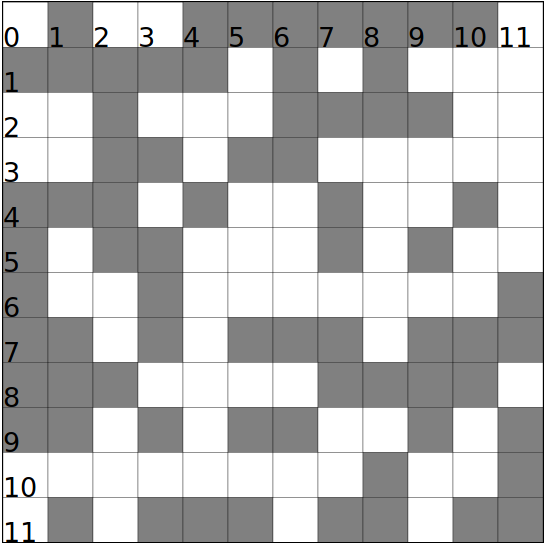
\includegraphics[width=.3\linewidth]{freq_for_2}
  \quad
  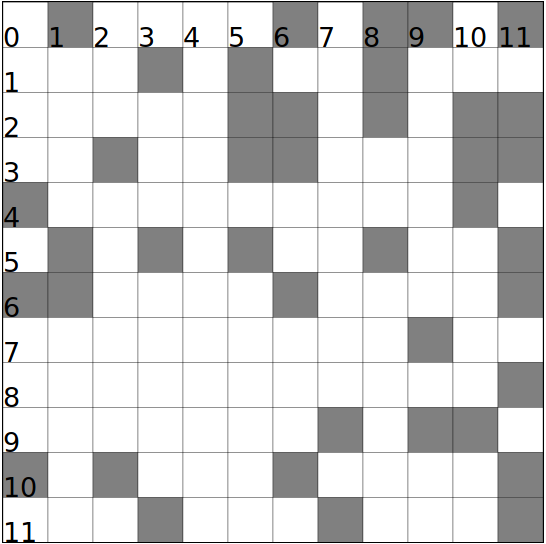
\includegraphics[width=.3\linewidth]{freq_for_4}
  \quad
  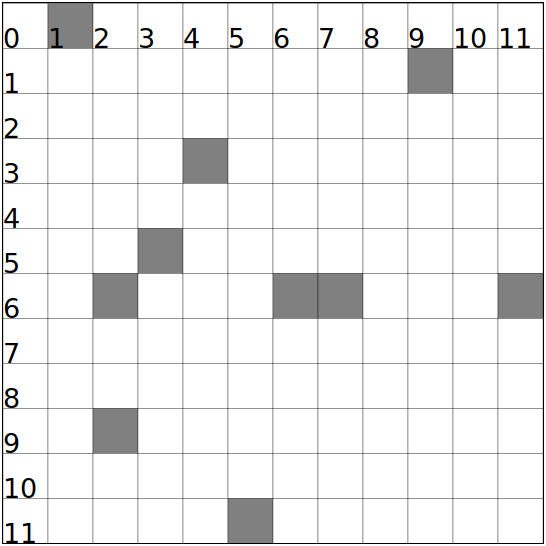
\includegraphics[width=.3\linewidth]{freq_for_16}\\
  \caption[Raster mit Frequenzparametern $freq = 2$, $freq = 4$ und $freq = 16$ im Wandgenerator.]{Raster mit Frequenzparametern $freq = 2$, $freq = 4$ und $freq = 16$ im Wandgenerator. Quelle: Eigenleistung}
  \label{fig:freq_param}
\end{figure}
Wir sehen also, dass mit dem Frequenzparameter $freq$ die Häufigkeit der unpassierbaren Wände geändert werden kann. In unserer Webapplikation haben wir für den Frequenzparameter $freq = 4$ ausgewählt, da dieser Wert ein gutes Gleichgewicht zwischen nicht zu viel unlösbaren Rastern und genügend Wänden ergibt.
\subsubsection{Generierung des Start-und Endpunkts}
Wählt man zwei zufällige passierbare Zellen als Start- und Endpunkt aus, erhält man ein Raster, mit dem man Pathfinding-Algorithmen anwenden kann. In unserer Webapplikation werden diese zwei Zellen farbig differenziert. Programmatikalisch handelt es sich um Zellen, die Wände sind und in Ziel- resp. Endpünkte umgewandelt werden. Die folgenden zwei Routinen\footnote{Die genaue Codestelle in der Webapplikation ist hier ersichtlich: \url{https://github.com/fuerbringer/bma/blob/master/src/maze.js\#L27}} wählen in einem gegebenen Raster einen Start- und einen Endpunkt aus.
\algblock[Name]{Let}{In}
\algblockdefx[NAME]{LET}{IN}%
[2][Unknown]{Let #1(#2)}%
{Ending}
\algblockdefx[NAME]{}{OTHEREND}%
[1]{Until (#1)}
\begin{algorithmic}[1]
  \Procedure{Startundendpunktgenerator}{$raster$}
  \State $frei$ ist eine leere Liste \Comment mögliche Zellen für den Start- und Endpunkt
  \For{$y \gets 0\ \textbf{to}\ $\textbf{count}(Zeilen von $raster$)}
    \For{$x \gets 0\ \textbf{to}\ $\textbf{count}(Zellen von $raster$ in der Zeile $y$)}
      \State $zelle \gets$ Zelle mit (x,y) in $raster$
      \If{$zelle$ ist keine Wand}
        \State $zelle$ der Liste $frei$ hinzufügen
      \EndIf
    \EndFor
  \EndFor
  \State $raster \gets \textsc{Punktemarkieren}(raster, frei)$
  \State \textbf{return} $raster$
  \EndProcedure

  \Procedure{Punktemarkieren}{$raster$, $frei$} \Comment Start- und Endpunkte markieren
  \State $startIndex \gets \floor{random(0, \textbf{count}(frei))}$ \Comment Zufallsindex für die Liste $frei$
  \Let
    \State $sx \gets$ $x$-Koordinate von $frei$ am Index $startIndex$
    \State $sy \gets$ $y$-Koordinate von $frei$ am Index $startIndex$
  \In \ Zelle in $raster$ bei $sx$ und $sy$ wird zum Startpunkt
  \State Element in $frei$ am Index $startIndex$ entfernen

  \State $endIndex \gets \floor{random(0, \textbf{count}(frei))}$ \Comment Zufallsindex für die Liste $frei$
  \Let
    \State $ex \gets$ $x$-Koordinate von $frei$ am Index $endIndex$
    \State $ey \gets$ $y$-Koordinate von $frei$ am Index $endIndex$
  \In \ Zelle in $raster$ bei $ex$ und $ey$ wird zum Endpunkt
  \State Element in $frei$ am Index $endIndex$ entfernen

  \State \textbf{return} $raster$
  \EndProcedure
\end{algorithmic}
Wendet man nun den Start- und Endpunktgenerator\footnote{Die genaue Codestelle in der Webapplikation ist hier ersichtlich: \url{https://github.com/fuerbringer/bma/blob/master/src/maze.js\#L27}} an Rastern mit Wänden (siehe Abbildung \ref{fig:freq_param}) an, so erhält man folgendes, ein für den PathFinder brauchbares, Raster mit Wänden und Start- und Endpunkt:
\begin{figure}[H]
  \centering
  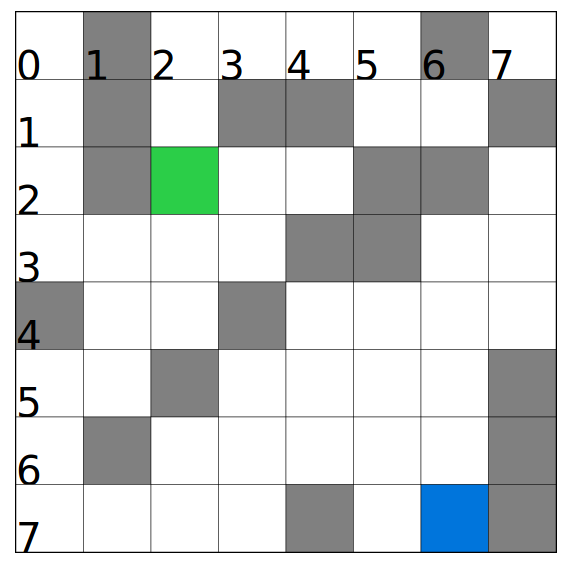
\includegraphics[width=8cm]{grid2}
  \caption[Ein von unserer Webapplikation generiertes $8\times8$ Raster mit Wänden und markierten Start- und Endpunkten.]{Ein von unserer Webapplikation generiertes $8\times8$ Raster mit Wänden und markierten Start- und Endpunkten. Quelle: Eigenleistung}
  \label{fig:grid2}
\end{figure}
Im letzten Schritt lässt man die PathFinder den Weg zwischen den markierten Start- und Enpunkten finden. Die Parameter, die man PathFinding.js dafür übergeben muss, sind grundsätzlich das Raster und die darin markierten Punkte, die als Start- und Ende dienen. Die markierten Punkte speichert man entweder im Start- und Endpunktgenerator zwischen oder man benutzt eine weitere Routine\footnote{Die genaue Codestelle in der Webapplikation ist hier ersichtlich: \url{https://github.com/fuerbringer/bma/blob/master/src/helper.js\#L15}}, die die Start- und Endpunkte aus einem Raster extrahiert:
\begin{algorithmic}[1]
  \Procedure{Startundendpunktfinden}{$raster$}
  \State $startPunkt \gets$ leeres Element
  \State $endPunkt \gets$ leeres Element
  \ForAll{$zeile \in raster$} \Comment $y$-Achse
    \ForAll{$zelle \in zeile$} \Comment $x$-Achse
    \If{Ist $zelle$ ein Startpunkt}
      \State $startPunk \gets zelle$ \Comment \textit{startPunkt} entspricht der aktuellen Zelle
    \ElsIf{Ist $zelle$ ein Endpunkt}
      \State $endPunk \gets zelle$ \Comment \textit{endPunkt} entspricht der aktuellen Zelle
    \EndIf
    \EndFor
  \EndFor
  \State \textbf{return} $startPunkt$ und $endPunkt$
  \EndProcedure
\end{algorithmic}
Übergibt man PathFinding.js nun die nötigen Parameter des Rasters und dessen Start-und Endpunkte, so erhält man den Weg von Start bis Ende. Wiederholt man dies mehrere Male mit verschiedenen Pathfindern, so ermöglicht man den direkten Vergleich der Pathfinding-Algorithmen. Dies ist eine wichtige Kernfunktion dieser Berufsmaturitätsarbeit.
\begin{figure}[H]
  \centering
  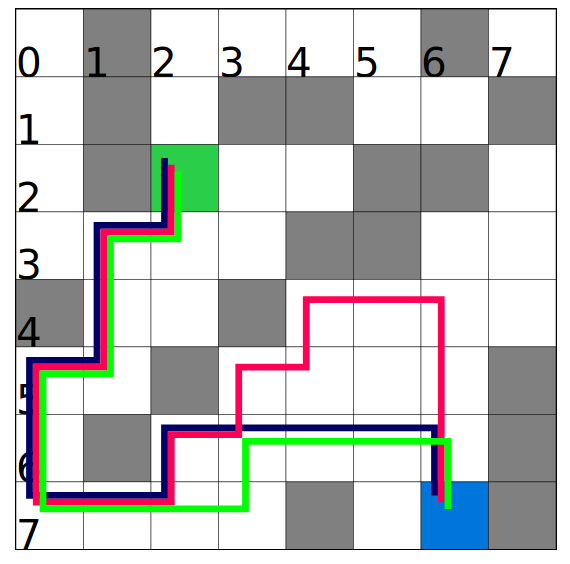
\includegraphics[width=8cm]{grid3}
  \caption[Ein von unserer Webapplikation generiertes $8\times8$ Raster mit Wänden und gelöstem Weg.]{Ein von unserer Webapplikation generiertes $8\times8$ Raster mit Wänden und gelöstem Weg. Quelle: Eigenleistung}
  \label{fig:grid3}
\end{figure}
\subsection{Auswertung und Merkmale}
Zur Auswertung werden Merkmale definiert, welche bei der Statistik relevant sind. Es folgen die drei wichtigsten Merkmale beim Vergleich der Pathfinder in der Webapplikation.
\subsubsection{Zurückgelegter Weg}
Der zurückgelegte Weg ist aus praktischer Sicht gesehen ein bedeutendes Merkmal, da man natürlich möchte, dass der resultierende Weg möglichst kurz ausfällt. 
Die Programmbibliothek PathFinding.js liefert den Weg in einer Liste mit einer Koordinate pro Element.
Daraus folgt, dass der Weg $s$ der Anzahl der Elemente der Liste entsprechen muss, wenn man nach PathFinding.js Sprünge oder Luftlinien ausschliest\footnote{Ein von PathFinding.js berechneter Weg: \url{https://pathfindingjs.readthedocs.io/en/latest/user-guide/getting-started/}}. 
Es gibt demnach keine Geraden, ausser zwischen zwei Benachbarten Punkten.
Diagonalen würden nach dieser Logik bei einem diagonalen Sprung als eine Wegeinheit gelten.
\[ s = n
\begin{cases}
  P_1(0,0),\\
  P_2(1,0),\\
  ...\\
  P_n(x,y)
\end{cases}
\]
\subsubsection{Operationen}
Ein Algorithmus, der für das gleiche Resultat weniger Schritte (Operationen) tätigen muss, ist grundsätzlich besser als ein anderer. Zur Erfassung der Anzahl Operationen mussten die internen Routinen der Programmbibliothek PathFinding.js angepasst werden, da sie solche Messungsmerkmale nicht standardmässig liefert. Dazu wurde der Quellcode von PathFinding.js kopiert\footnote{Diesen Prozess nennt man bei freier Software ``Forking''.} und in die Routinen der drei ausgewählten Pathfinder im äusseren und inneren Loop eingefügt. Folgende Dateien\footnote{Die genauen Anpassungen sind unter dem folgenden Link verfügbar: \url{https://github.com/fuerbringer/PathFinding.js/commit/51034158638ad7aaa9c5142a827bd4d3de2b8786\#diff-22360b18a43ac33ae398e44b998101c7}} wurden dafür angepasst:
\begin{itemize}
\item{src/finders/AStarFinder.js}
\item{src/finders/BreadthFirstFinder.js}
\end{itemize}
Zu beachten ist, dass die Datei des BestFirstFinders nicht angepasst werden musste, da dieser auf dem A*-Finder basiert und somit alle Änderungen vom A*-Finder vererbt.
\subsubsection{Rechenzeit}
Ein bedeutendes Merkmal ist die Rechenzeit, also die Zeit, in der der Pathfinder seine Arbeit verrichtet hat. 
Um diese zu berechnen, wird unmittelbar vor der Ausführung der Wegfindungsroutine des Pathfinders der Zeitstempel $t_0$ der jetzigen Zeit zwischengespeichert und danach vom Pathfinder die Arbeit verrichtet. 
Direkt nach dem Beenden der Wegfindung wird ein zweites Mal ein Zeitstempel $t_1$ zwischengespeichert. Die Differenz ergibt die Zeit $t$ in Millisekunden\footnote{Die Einheit Millisekunden ergibt sich aus der Schnittstelle \texttt{Performance.now()} von JavaScript}, die für die Berechnung benötigt wurde.
\begin{equation}
  t = t_1 - t_0
\end{equation}
Die Werte $t$ sind pro Pathfinder in der Webapplikation unter ``Messung für diesen Einzelversuch:'' unter dem Raster ersichtlich. Diese Berechnung demnach pro Durchlauf dreimal getätigt.
\\\\
Aus diesen drei Merkmalen folgen zusammengefasst die in unserer Webapplikation vermessenen Werte der Pathfinding-Algorithmen.
\begin{figure}[H]
  \centering
  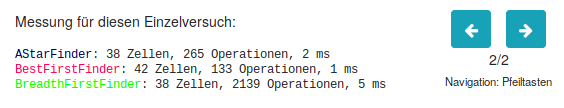
\includegraphics[width=10cm]{measurements_single}
  \caption[Ausschnitt aus dem Pathfinding-Vergleicher für einzelne Vergleiche.]{Vergleicherausschnitt. Quelle: Eigenleistung}
  \label{fig:gui_konzept_comparator}
\end{figure}


%%%%%%%%%%%%%%%%%%%%%%%%%%%%%%%%%%%%%%%%%%%%%%%%%%%%%%%%%%%%%%%%%%%%%%%%%%%%%%%%
\chapter{Schluss}
%TODO

\chapter{Anhang}
\section{Screenshots der Webapplikation}
%TODO Willkommen Scrot
%TODO Einleitung Scrot
%TODO Visualisierer Scrot
\subsection{Pathfinder-Vergleicher}
\begin{figure}[h]
  \centering
  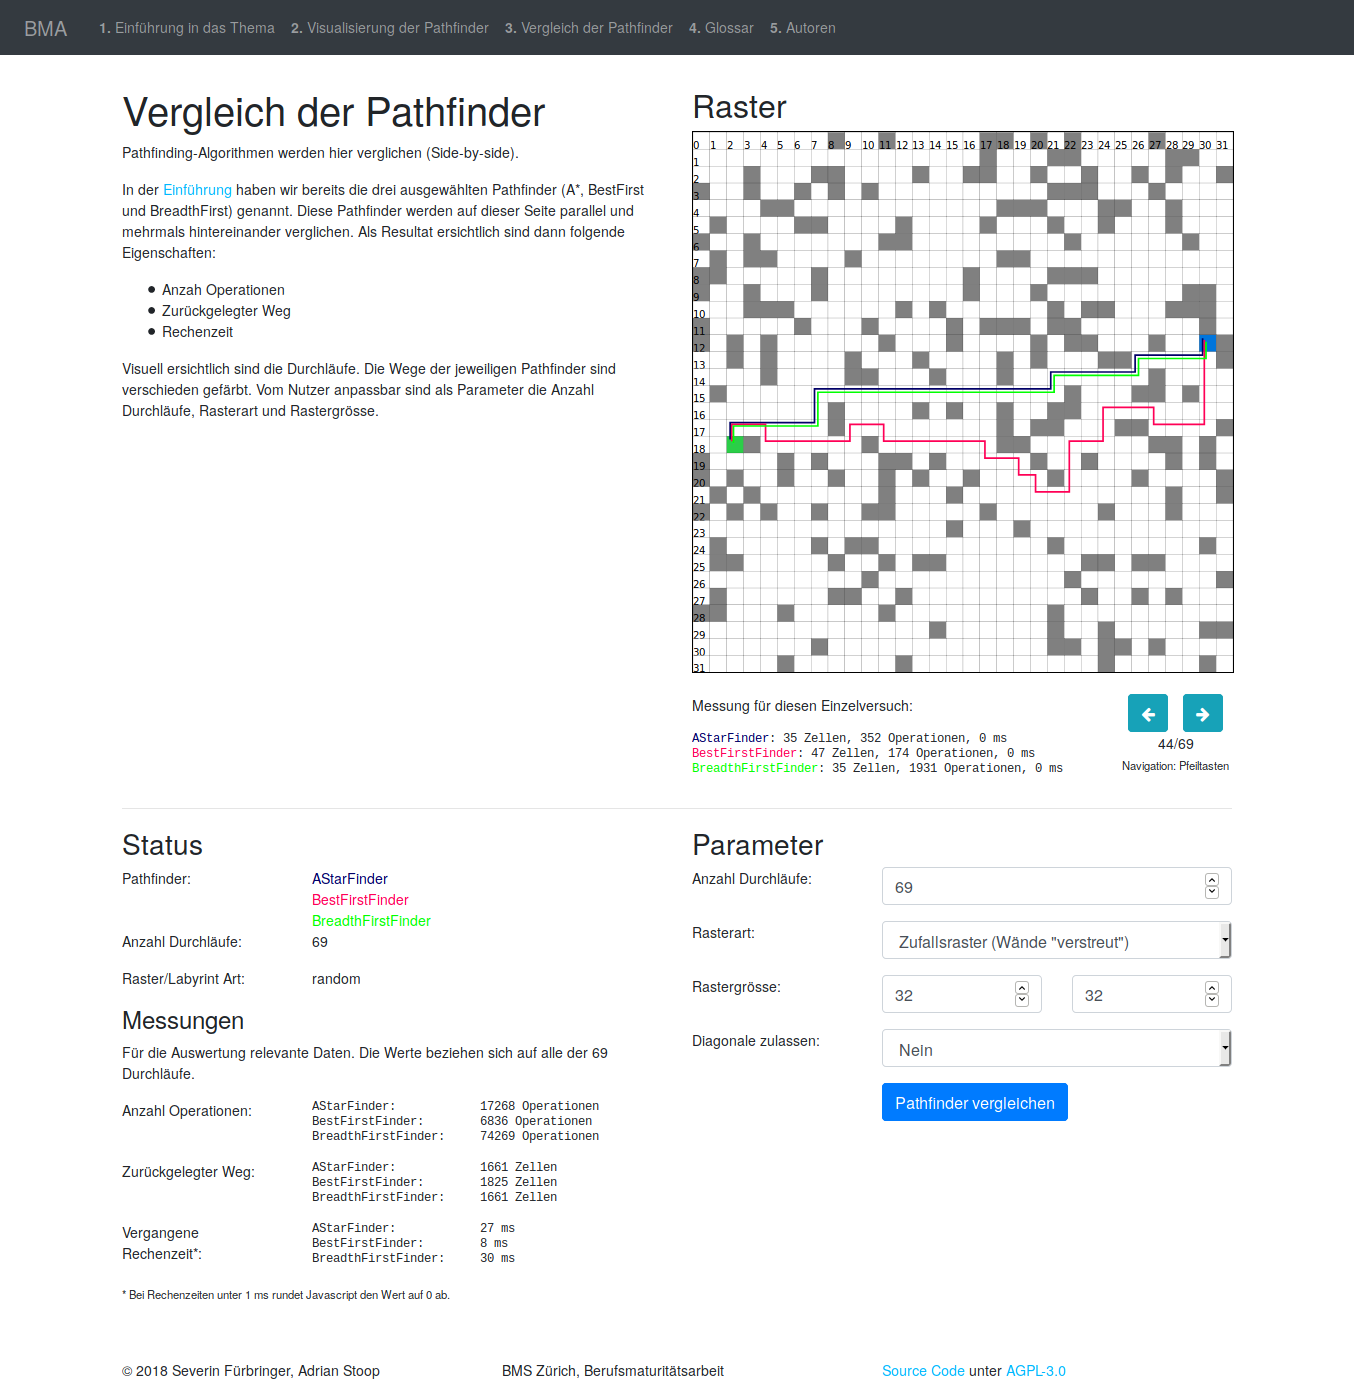
\includegraphics[width=14cm]{3_full}
  \caption[Ein vollständiger Screenshot des Pathfinder-Vergleichers.]{Pathfinder-Vergleicher-Page. Quelle: Eigenleistung}
  \label{fig:comparator_screenshot}
\end{figure}

\section{Danksagung}
\blindtext

\subsection{Schriftsetzung}
Die Schriftsetzung wurde durch die freie Software \LaTeX\  und deren Autoren Leslie Lamport et. al. ermöglicht.

\chapter{Glossar}
\section*{Fachwörter- und Begriffsverzeichnis}
In diesem Kapitel werden wichtige Wörter aus der Fachsprache erklärt, die in unserer Arbeit oftmals vorkommen.
\paragraph{A*} Sprich ``A Star''. Ein Pathfinding Algorithmus (siehe Fachbegriff Algorithmus). Dieser nutzt zusätzlich heuristische Mittel, um den Weg zu berechnen (siehe Heuristik).
\paragraph{Algorithmus} Ein Ablauf, Prozess oder Programm, der eine Liste mit Anweisungen schrittweise befolgt, um Daten umzuwandeln.
\paragraph{Back-End} Der Server---mit guten Systemtechnikern rund um die Uhr stellt das Back-End die Website unter einer URL, wie \texttt{bma.fuerbringer.info}, zur Verfügung.
\paragraph{BestFirstFinder} Ein Pathfinding-Algorithmus. Nicht zu verwechseln mit dem BreadthFirstFinder.
\paragraph{BreadthFirstFinder} Ein Pathfinding-Algorithmus. Nicht zu verwechseln mit dem BreadthFirstFinder.
\paragraph{Dijkstra} Ein Pathfinding Algorithmus (siehe Fachbegriff Algorithmus). Dieser nutzt keine heuristische Mittel und kommt in unserer Arbeit nicht direkt vor.
\paragraph{Front-End} Der Browser---der Teil einer Website oder Webapplikation, den der Benutzer sieht und mit dem er interagiert. In unserem Fall werden die wichtigsten Berechnungen im Front-End verrichtet.
\paragraph{Heuristik} Hilfsalgorithmus, unter anderem für Pathfinder, der zusätzlich hilft zwischen einzelnen Schritten die Kosten für eine mögliche Operation einzuschätzen.
\paragraph{Matrix} Anordnung von Elementen. In unserem Fall ein zweidimensionales Raster, in dem Wände, Korridore und Wege platziert sind.
\paragraph{Operationen} Eine ``Operation'' beschreibt in unserem Fall einen Zyklus eines Pathfinders. Je mehr Zyklen ein Pathfinder in Relation zu einem anderen benötigt, desto weniger effizient ist er.
\paragraph{Parameter} Die Randbedingungen für einen Durchlauf bzw. ein Experiment.
\paragraph{PathFinding.js} Die Zentrale Programmbibliothek, deren Pathfinder Implementationen wir in unserer Webapplikation nutzen.
\paragraph{Pathfinder} Eine Art Algorithmus, der in einem gegebenen Raum mit eingezeichnetem Start- und Endpunkt den schnellsten weg Findet.
\paragraph{recbacktracker} ``Recursive Backtracker, ein Labyrinthalgorithmus, den wir in unserer Webapplikation zur Generierung von perfekten (immer lösbaren) Labyrinthen verwenden. Dieser Algorithmus kommt im Vergleicher nicht zum Zug.
\paragraph{Pseudocode} Definiert einen Algorithmus schriftlich in einer allgemein verständlichen Sprache, damit dieser in beliebigen Programmiersprachen umgesetzt werden kann.
\paragraph{PHP} Eine freie serverseitige Programmiersprache, die seit über zwei Jahrzehnten einen hohen Marktanteil hat.
\paragraph{JavaScript} Nicht zu verwechseln mit Java. Eine clientseitige Programmiersprache, die in jedem Browser integriert ist. Sie wird hauptsächlich zwecks der Interaktivität benutzt. 
\paragraph{Implementieren/Implementation} Im Kontext der Software wird damit die Planung und Entwicklung des Quellcodes bezeichnet.
\paragraph{Pixelmatrizen} Eine Liste mit Pixeldaten, die zum Beispiel bei Computergrafikapplikationen gebraucht wird. Der ``Inhalt'' des Bildschirm kann ganzheitlich in einer Pixelmatrix abgelegt werden.
\paragraph{Prozedural} Beschreibt programme, die schrittartig ablaufen.
\paragraph{Routine} Unter diesem Begriff kann man im Rahmen dieser Arbeit einen Teil eines Algorithmus, einer Funktion oder einer Prozedur verstehen.
\paragraph{Unix und GNU/Linux} Betriebssysteme abstammend vom AT\&T UNIX.


% END THESIS CONTENT
%%%%%%%%%%%%%%%%%%%%%%%%%%%%%%%%%%%%%%%%%%%%%%%%%%%%%%%%%%%%%%%%%%%%%%%%%%%%%%%%

\clearpage

\begin{thebibliography}{9}
\bibitem{pfjs}
  Xueqiao Xu et al.,
  \textit{PathFinding.js},
  \url{https://github.com/qiao/PathFinding.js},
  Quellcode auf GitHub,
  Letzter Aufruf: \today
\bibitem{cuishi2011}
  Xiao, Cui; Hao Shi,
  \textit{A*-based Pathfinding in Modern Computer Games},
  IJCSNS International Journal of Computer Science and Network Security, VOL.11 No.1,
  Januar 2011.
\bibitem{bma}
  Fürbringer, Severin; Stoop, Adrian,
  \textit{BMA Quellcode},
  \url{https://github.com/fuerbringer/bma},
  \today
\bibitem{bmaonline}
  Fürbringer, Severin; Stoop, Adrian,
  \textit{BMA-Webapplikation},
  \url{https://bma.fuerbringer.info},
  \today
\end{thebibliography}


\listoffigures

\end{document}
